% chktex-file 44

\documentclass[a4paper,12pt]{article}
\usepackage[utf8]{inputenc}
\usepackage[russian]{babel}
\usepackage{geometry}
\usepackage{amsthm}
\usepackage[dvipsnames]{xcolor}
\usepackage{framed}
\usepackage{booktabs}
\usepackage{array}
\usepackage{amssymb}
\usepackage{adjustbox}
\usepackage{makecell}
\usepackage{float}
\usepackage{graphicx}

\definecolor{shadecolor}{RGB}{245,245,247} 
\geometry{left=2cm, right=2cm, top=2cm, bottom=2cm}

\title{Модель №.3. \\ Магнитные колебания. \\ Связанные маятники }
\author{Ким В.Р., Вишневский С.А \\ Группа M3207 }
\date{}

\theoremstyle{definition}
\newtheorem*{task}{Задание}\setlength{\parindent}{0pt}

\newenvironment{solution}
{\begin{shaded}\textbf{Решение:}\par\setlength{\parindent}{0pt}}
{\end{shaded}}

\newenvironment{answer}
{\par\noindent\textbf{Ответ:} }
{\par}

\begin{document}
\maketitle

\begin{task}
    Два одинаковых математических маятника, связанных пружиной с коэффициентом 
    жёсткости \(k\) на расстоянии \(L_1\) от точки крепления маятников. 
    Точки крепления обоих связанных маятников находятся на одном уровне. 
    Оба математических маятника имеют одинаковые длины подвеса \(L\) и массы \(m\) 
    (см. Рис.). 
    Сила сопротивления для каждого маятника прямо пропорциональна скорости. 
    Коэффициент затухания каждого маятника равен \(\beta\). Для заданных начальных 
    отклонений построить графики зависимостей углов и скоростей от времени 
    для каждого маятника. Найти нормальные частоты. 
    Параметры должны задаваться.

    \begin{figure}[H]
        \centering
        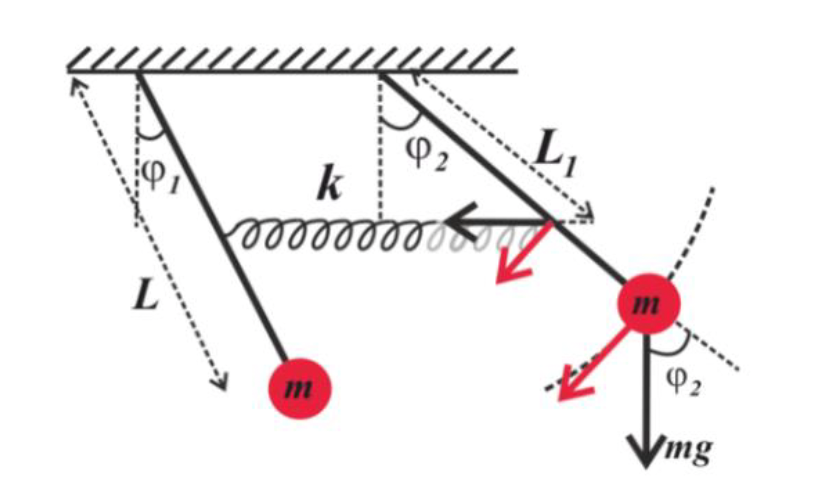
\includegraphics[width=0.5\textwidth]{task.png}  
    \end{figure}

\end{task}


\end{document}